From the previous discussion, we summarise that both one-dimensional and two-dimensional indexes requires to learn a function from a one-dimensional array. 
\begin{enumerate}
	\item In one dimensional data, the learned function is used directly as an approximation to the CDF. We use a fully connected neural network or a recursive model to learn such function.
	\item In two dimensional data, the learned function is used to predict the corresponding shard. We use a piecewise linear function to achieve this task.
\end{enumerate}

These models in our previous chapters have their shortcomings:

\begin{enumerate}
	\item The fully connected neural network (with ReLU as activation functions) is essentially a continuous piecewise linear function. The training of such neural network is unstable and highly dependent on the initial values, well-tuned hyper-parameters, etc. Meanwhile, it requires more work if we want to ensure the monotonicity.
	\item The recursive model takes more memory than a single neural network, and there are many more parameters to tune than neural network. 
	\item The training method for a piecewise linear function is an iteration-based method. If we choose a large number of break points, then the training time will be long.
\end{enumerate}

In fact, in order to train the piecewise linear function, we only need to know either the slope of each segments or the position of the breakpoints. If we know any one of them, we can learn the other in a closed form, as we shown in the shard prediction section. In this chapter, we present a method to learn the position of breakpoints.

Learning the position of breakpoints can be regarded as a binary point-wise classification problem. That means, for each point in our $X$, we want to learn to classify it to be $1$ if it is a breakpoint, otherwise we want it to be $0$. Then we classify all the points in our $X$ and each point is classified to be $1$ with a confidence. Afterwards, we only need to filter the top-$K$ points to be the breakpoints.

This task is similar to the image segmentation in computer vision, which essentially tries to classify every pixel in the image. One successful technique in image segmentation is by using the convolution and convolution transpose network \cite{long2015fully}. Inspired by this, we propose a similar network to perform binary point-wise classification. In this chapter, we describe the steps of using convolutional neural network to find breakpoints in a one-dimensional array.

\section{Problem Formation}

Assume that we have the keys $X$ and their corresponding pages $Y$, the problem can be formulated and divided into the following subproblems:

\begin{enumerate}
	\item How do we prepare the training labels $L$ that represents the break points?
	\item What kind of neural networks is capable of classifying each points in the training input $X$ and $Y$?
	\item After predicting the break points, how do we proceed to train linear function on each segment? 
\end{enumerate}

\section{Training}

\subsection{Dataset}

The dataset we used in the convolutional neural network is manually synthesised as well. We use the following steps to generate the training dataset:

\begin{enumerate}
	\item Similar to the dataset we used in recursive model, we first generate $X$ by randomly sampling from a certain distribution. Then we assign the keys into different pages according to a preset parameter $N_{page}$. We call the generated pages as $Y$. After this step, we get a two-dimensional matrix.
	\item Then we calculate the positions of breakpoints by the iteration-based approach described in the \textit{Shard Prediction} section.
	\item Afterwards, we iterate over all the calculated breakpoints and find the closest point to it in $X$. We call the set of closest points as $B$ and we can generate the training labels as
	\begin{equation}
		l=\begin{cases}
			1 & x\in B \\
			0 & \text{otherwise} 
		\end{cases}
	\end{equation}
\end{enumerate}

In addition to the above steps, we could also generate several dataset from several different distributions, and then concatenate them such that the training dataset contains samples from different distributions.

After these steps, we get the training input as $[X, Y]$ and the training label as $L$. Assume there are $N$ keys in total, then the training input is a $N\times 2$ matrix and the training label is a $N\times 1$ vector.

\subsection{Fully Convolutional Network}

Convolution is an operation that makes the input smaller, which makes it impossible to perform point-wise classification. Hence, we use the convolution transpose (also called deconvolution) to make the input larger. We manually set up the hyper-parameters (e.g. the kernel size of convolution operation) in the neural network such that the output has a shape of $N\times 1$. In our experiments, we use the neural network illustrated as Fig. \ref{fig:5_fcn}.

\begin{figure}
\centering
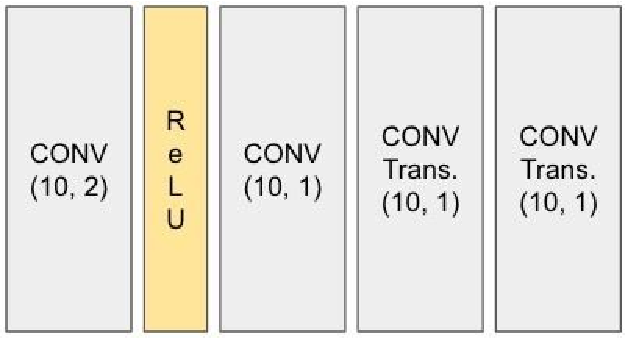
\includegraphics[width=0.4\textwidth]{graphs/fcn/fcn.pdf}
\caption{Illustration of the structure of fully convolutional network, in which the yellow rectangle represents the activation function and other grey rectangles represents convolution and convolution transpose operations. The $(10, 2)$ and $(10, 1)$ represent the kernel size of the convolution operation}
\label{fig:5_fcn}
\end{figure}

With this neural network, we can get an output of the shape $N\times 1$. The expected output represents the probability that this position is a breakpoint.

We can train the neural network with standard gradient descent approach. During the training process, we try to minimise the mean square distance between the predicted output $\hat{L}$ and the labels $L$.


\subsection{Training of Linear Functions}

After getting the predicted output, we then find the largest $K+1$ positions from the predicted output $\hat{L}$. We call these $K$ elements as $\boldsymbol{\beta}=(\beta_0, \beta_1, \cdots, \beta_K)$. Then we want to train a piecewise linear function described as 

\begin{equation}
	y=\begin{cases}
		\overline{\alpha} + \alpha_0(x-\beta_0) & \beta_0\leq x<\beta_1 \\
		\overline{\alpha} + \alpha_0(x-\beta_0) + \alpha_1(x-\beta_1) & \beta_1\leq x<\beta_2 \\
		\cdots \\
		\overline{\alpha}+ \alpha_0(x-\beta_0) + \alpha_1(x-\beta_1)+\cdots+\alpha_{K}(x-\beta_K) & \beta_K\leq x
	\end{cases}
\end{equation}

Since $\boldsymbol{\beta}$ is fixed, we only need to calculate $\boldsymbol{\alpha}=(\overline{\alpha},\alpha_1,\alpha_2,\cdots,\alpha_K)$, which can be considered as the solution of the linear equation $\boldsymbol{A}\boldsymbol{\alpha}=\boldsymbol{y}$, where

\begin{equation}
	\boldsymbol{A}=\left[\begin{array}{ccccc}
1 & x_{0}-\beta_{0} & \left(x_{0}-\beta_{1}\right) 1_{x_{0} \geq \beta_{1}} & \ldots & \left(x_{0}-\beta_{K}\right) 1_{x_{0} \geq \beta_{K}} \\
1 & x_{1}-\beta_{0} & \left(x_{1}-\beta_{1}\right) 1_{x_{1} \geq \beta_{1}} & \ldots & \left(x_{1}-\beta_{K}\right) 1_{x_{1} \geq \beta_{K}} \\
\vdots & \vdots & \vdots & \ddots & \vdots \\
1 & x_{N}-\beta_{0} & \left(x_{N}-\beta_{1}\right) 1_{x_{N} \geq \beta_{1}} & \cdots & \left(x_{N}-\beta_{K}\right) 1_{x_{N} \geq \beta_{K}}
\end{array}\right]
\end{equation}

where $1_{x_i\geq \beta_j}$ equals to $1$ if $x_i\geq \beta_j$. Otherwise it equals to $0$.

The by applying least square method, we get 

\begin{equation}
	\boldsymbol{\alpha}=(\boldsymbol{A}^T\boldsymbol{A})^{-1}\boldsymbol{A}\boldsymbol{y}
\end{equation}

The calculated $\boldsymbol{\alpha}$ and $\boldsymbol{\beta}$ are what we need to define the piecewise linear functions. With these steps, we could calculate them within a fixed number of computations. 

\section{Experiment}

We first present the break points that we found with the fully convolutional network as in Fig. \ref{fig:fcn_betas_found}.

\begin{figure}[t]
\begin{subfigure}[b]{0.5\textwidth}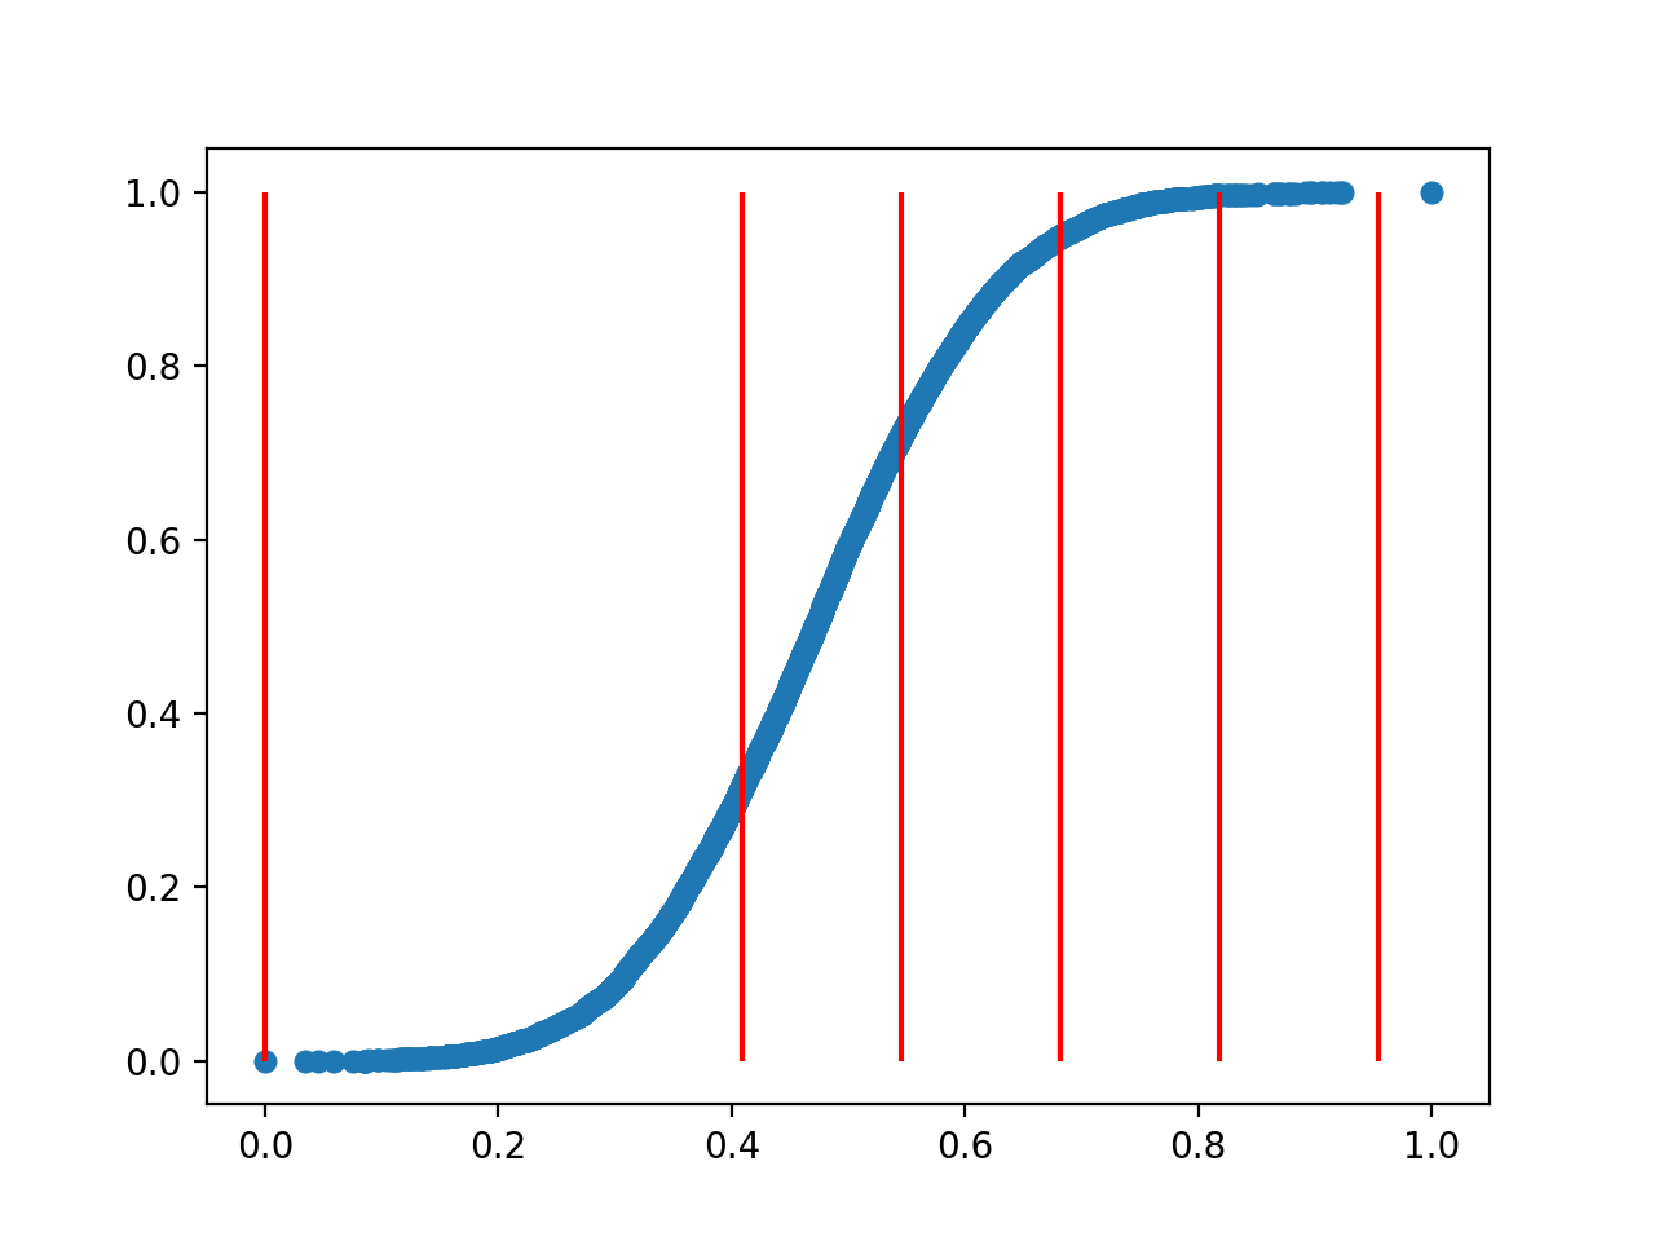
\includegraphics[width=8cm]{graphs/fcn/normal}
\caption{Normal Distribution}
\end{subfigure}	
\hfill
\begin{subfigure}[b]{0.5\textwidth}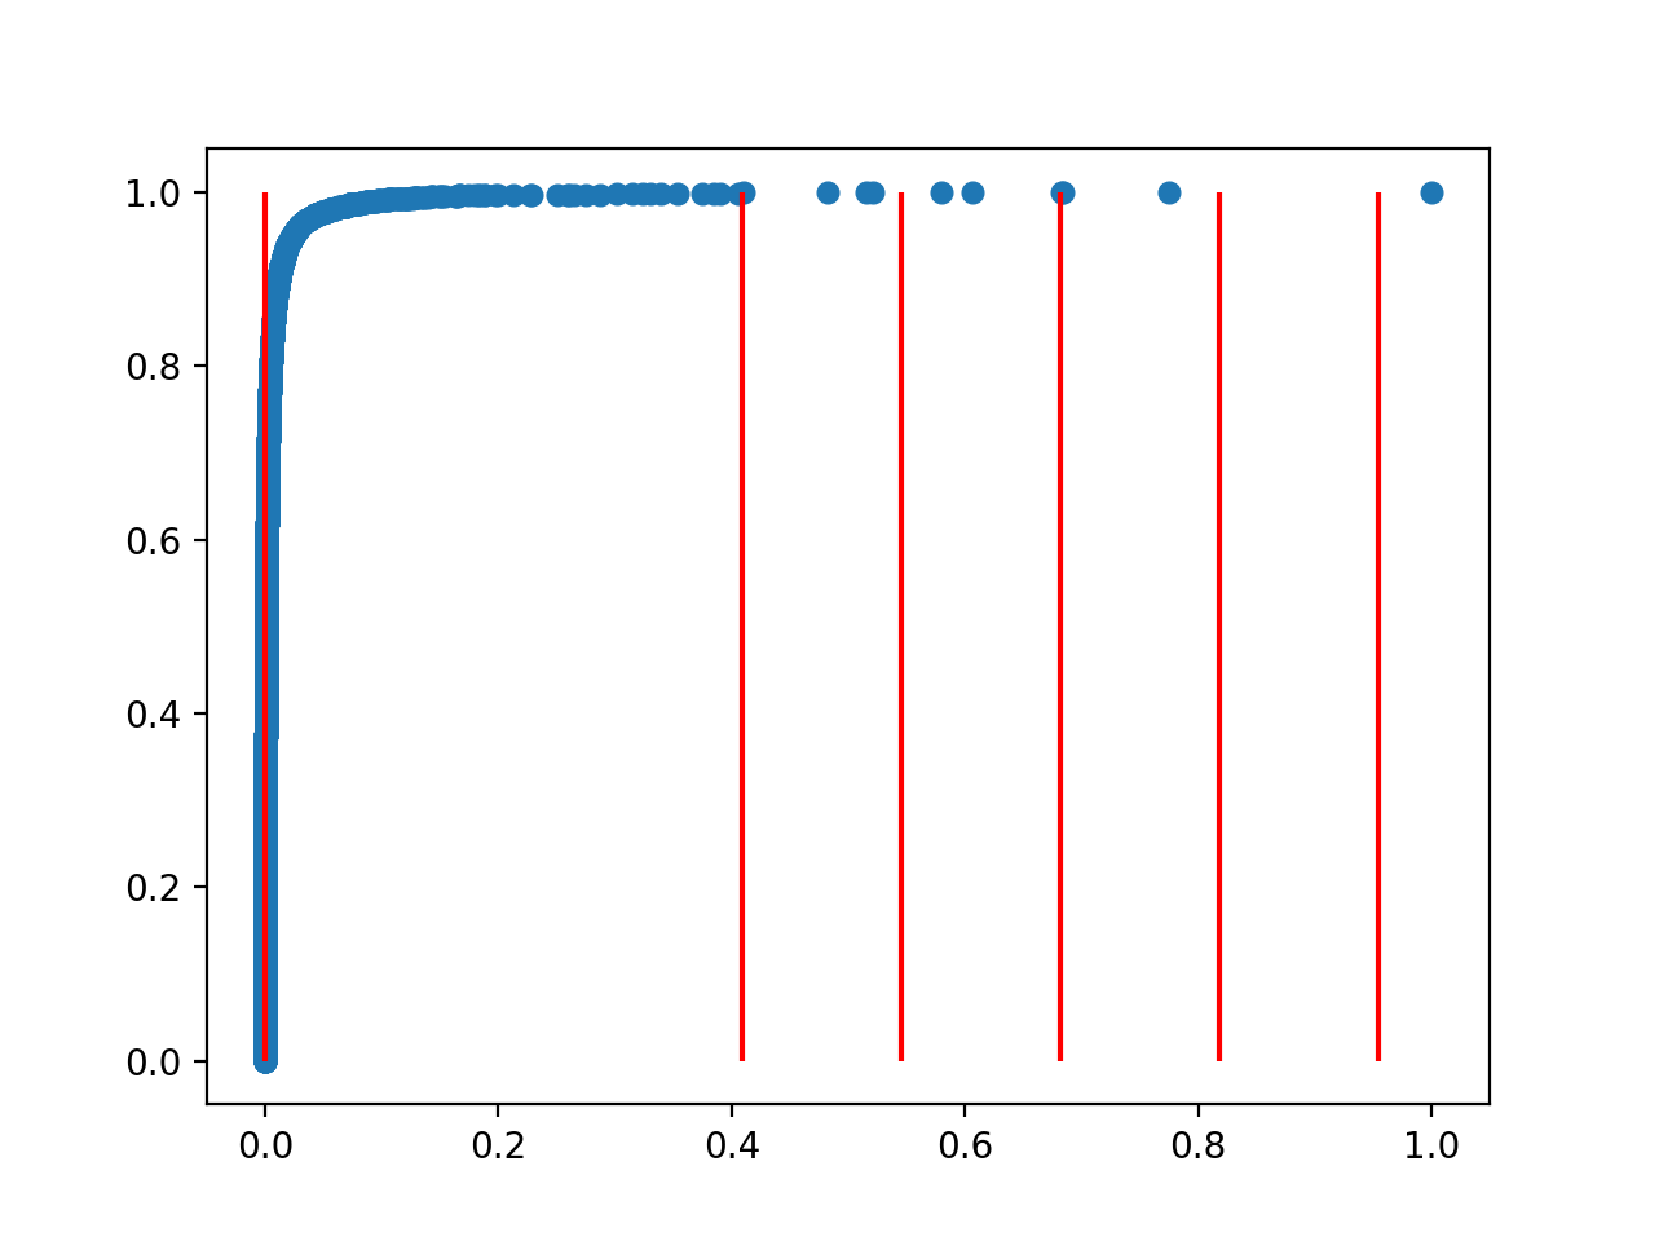
\includegraphics[width=8cm]{graphs/fcn/lognormal}
\caption{Lognormal Distribution}
\end{subfigure}
\caption{The break points found by the fully convolutional neural network}
\label{fig:fcn_betas_found}
\end{figure}

\section{Applications and Future Work}

The approach we described above can be used in both one-dimensional and two-dimensional data. In one-dimensional case, the learned piecewise function can be used directly as the approximation for the CDF. In the two-dimensional case, this approach can be used to improve the training speed of shard prediction function.

In future, there might be some possibilities in exploring in the following directions:

\begin{enumerate}
	\item Concatenate more distributions and explore if the convolutional model has actually learned the patterns for break points.
	\item Investigate the hyper-parameters in the fully convolutional neural network.
	\item We can find the break points not only for linear piecewise functions, but also polynomials etc. It might be possible for the convolutional neural network to learn the patterns of break points under different functions for each segment. That means, we may extend the binary classification task into a multi-categories classification task where each category represents a type of functions.
\end{enumerate}





































